\documentclass[a4paper,11pt]{article}

\usepackage[T1]{fontenc}
\usepackage[utf8]{inputenc}
\usepackage{graphicx}
\usepackage{xcolor}
\usepackage[section]{placeins}

\renewcommand\familydefault{\sfdefault}
\usepackage{tgheros}

\usepackage{amsmath,amssymb,amsthm,textcomp}
\usepackage{enumerate}
\usepackage{multicol}
\usepackage{tikz}

\usepackage{geometry}
\geometry{left=25mm,right=25mm,%
bindingoffset=0mm, top=20mm,bottom=20mm}


\linespread{1.3}

\newcommand{\linia}{\rule{\linewidth}{0.5pt}}

% custom theorems if needed
\newtheoremstyle{mytheor}
    {1ex}{1ex}{\normalfont}{0pt}{\scshape}{.}{1ex}
    {{\thmname{#1 }}{\thmnumber{#2}}{\thmnote{ (#3)}}}

\theoremstyle{mytheor}
\newtheorem{defi}{Definition}

% my own titles
\makeatletter
\renewcommand{\maketitle}{
\begin{center}
\vspace{2ex}
{\huge \textsc{\@title}}
\vspace{1ex}
\\
\linia\\
\@author \hfill \@date
\vspace{4ex}
\end{center}
}
\makeatother
%%%

% custom footers and headers
\usepackage{fancyhdr}
\pagestyle{fancy}
\lhead{}
\chead{}
\rhead{}
\lfoot{}
\cfoot{}
\rfoot{\thepage}
\renewcommand{\headrulewidth}{0pt}
\renewcommand{\footrulewidth}{0pt}
%

% code listing settings
\usepackage{listings}
\lstset{
    language=Python,
    basicstyle=\ttfamily\small,
    aboveskip={1.0\baselineskip},
    belowskip={1.0\baselineskip},
    columns=fixed,
    extendedchars=true,
    breaklines=true,
    tabsize=4,
    prebreak=\raisebox{0ex}[0ex][0ex]{\ensuremath{\hookleftarrow}},
    frame=lines,
    showtabs=false,
    showspaces=false,
    showstringspaces=false,
    keywordstyle=\color[rgb]{0.627,0.126,0.941},
    commentstyle=\color[rgb]{0.133,0.545,0.133},
    stringstyle=\color[rgb]{01,0,0},
    numbers=left,
    numberstyle=\small,
    stepnumber=1,
    numbersep=10pt,
    captionpos=t,
    escapeinside={\%*}{*)}
}

%%%----------%%%----------%%%----------%%%----------%%%

\begin{document}

\title{CS 426 Parallel Computing Project 3 Report}

\author{Bartu Atabek - 21602229}

\date{30/04/2020}

\maketitle

\section{Parallelization Strategy}
\subsection{Parallelization strategy used in the two parts. (You can use any parallelization strategy that scales up.)}

This project concerns multiplication of a sparse matrix with a vector. I implemented the operation xi+1 = Axi, where A is a sparse matrix and x is the vector. We were instructed to store result of the product of A and x into x at the end of ith iteration and use it in the i+1th iteration).
\newline
\newline
From the given test matrices we were instructed to represent the sparse matrix data using the Compressed row storage (CRS) format where we are storing the nonzero elements row-wise. Three vectors are needed:
\begin{itemize}
	\item \textbf{values array:} float vector storing the matrix elements
	\item \textbf{col\_ind array:} int vector storing the column indices of the matrix elements
	\item \textbf{row\_ptr array:} int vector pointing to the first elements of each row
\end{itemize}

With the given structures for my parallelization strategy I computed the resulting vector x element-by-element:

\begin{equation}
    y(k) =\sum_{i= row_ptr(k)}^{row_ptr(k+1)-1}a(i)\cdot x*({col_ind(i}))
\end{equation}

This is a ‘sparse’ dot product. One vector is stored contiguously
(stride one), the other vector is scattered in memory. In this equation we assume that row ptr(N) points to the memory location right after the last element of a, i.e. right after the last element of the last row of A.

\begin{equation}
col.ind(i_1) \neq col.ind(i_2) for
\end{equation}
\begin{equation}
row.ptr(k) \leq i_1 <  i_2 < row.ptr(k+1)
\end{equation}

With CRS parallelization over rows is straightforward in which for each iteration I used the '\#pragma omp for' for-loop to iterate through the values and used '\#pragma omp atomic' to protect a single update to a shared variable to store the multiplication results. Afterwards I used '\#pragma omp barrier' so that no thread can proceed past a barrier until all the other threads have arrived. By using it I was able to synchronize the threads in order to gather all the multiplication results into the 'x' vector.

\section{Figures for Each Test Matrix}
\subsection{The parallel running time, speedup, and efficiency of my OpenMP implementation for test-matrix "fidapm08.mtx"}

\begin{figure}[!htb]
    \centering
    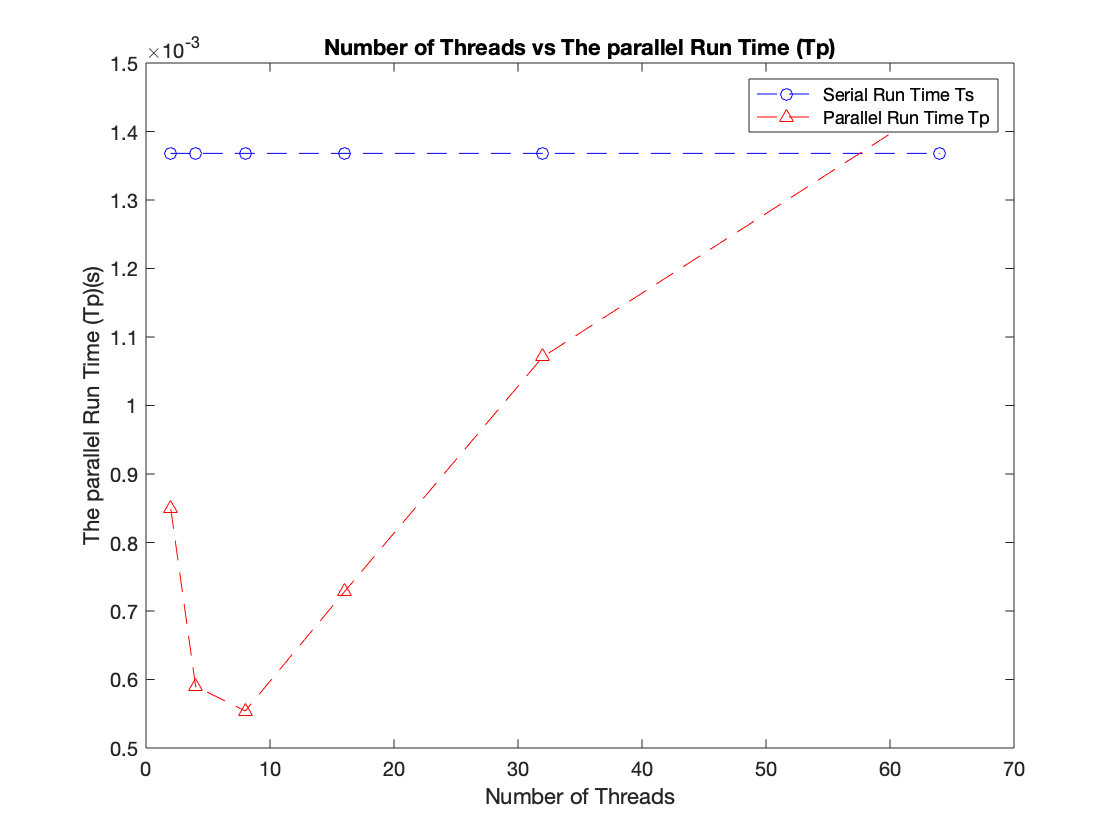
\includegraphics[width=0.75\textwidth]{f1}
    \caption{Serial vs Parallel Run-time comparison of sparse matrix vector multiplication on test-matrix "fidapm08.mtx" where number of threads for parallel execution is between 2 and 64.}
\end{figure}

\begin{figure}[!htb]
    \centering
    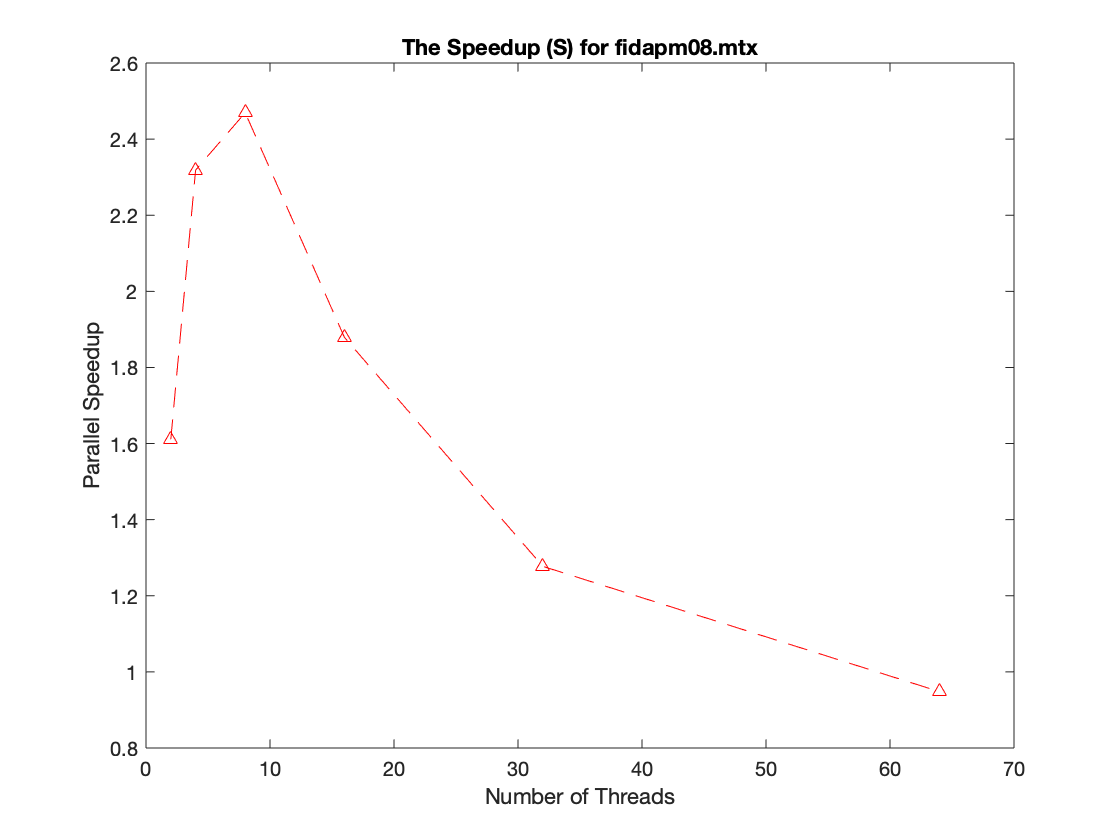
\includegraphics[width=0.75\textwidth]{s1}
    \caption{The speedup S on test-matrix "fidapm08.mtx" where number of threads for parallel execution is between 2 and 64.}
\end{figure}

\begin{figure}[!htb]
    \centering
    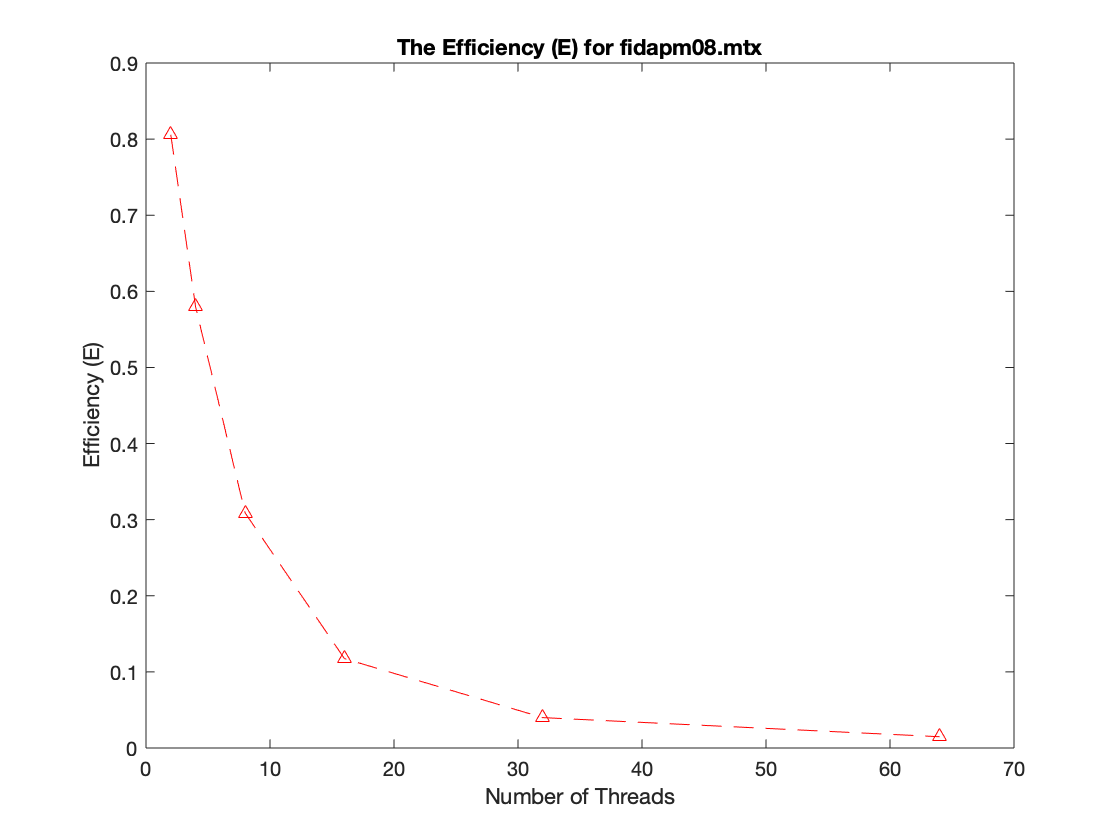
\includegraphics[width=0.75\textwidth]{e1}
    \caption{The efficiency E on test-matrix "fidapm08.mtx" where number of threads for parallel execution is between 2 and 64.}
\end{figure}

\FloatBarrier
\subsection{The parallel running time, speedup, and efficiency of my OpenMP implementation for test-matrix "fidapm11.mtx"}

\begin{figure}[!htb]
    \centering
    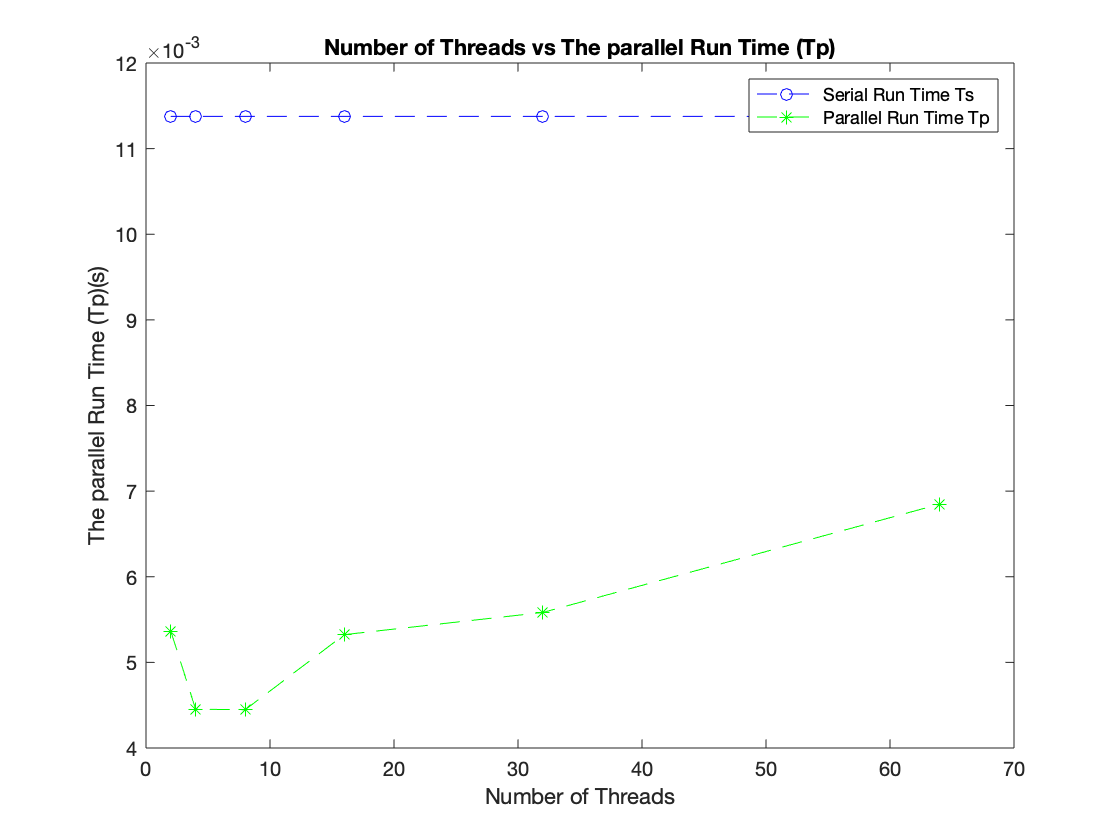
\includegraphics[width=0.75\textwidth]{f2}
    \caption{Serial vs Parallel Run-time comparison of sparse matrix vector multiplication on test-matrix "fidapm11.mtx" where number of threads for parallel execution is between 2 and 64.}
\end{figure}

\begin{figure}[!htb]
    \centering
    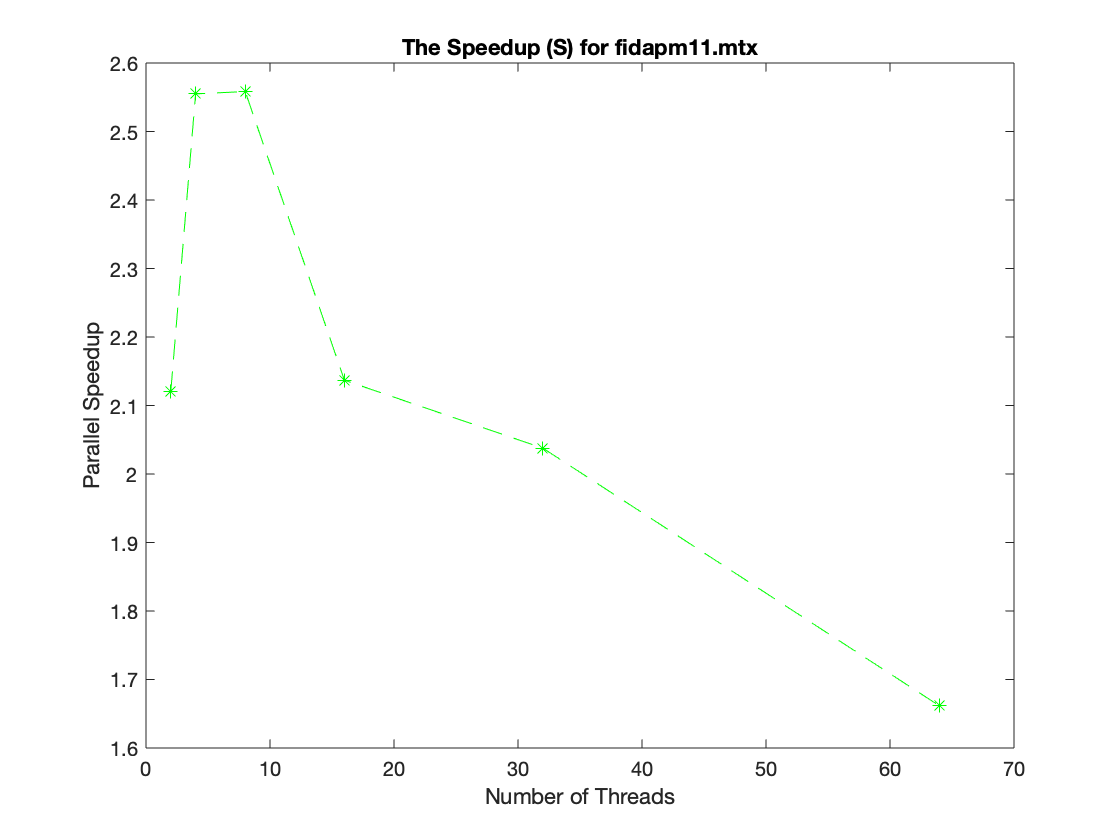
\includegraphics[width=0.75\textwidth]{s2}
    \caption{The speedup S on test-matrix "fidapm11.mtx" where number of threads for parallel execution is between 2 and 64.}
\end{figure}

\begin{figure}[!htb]
    \centering
    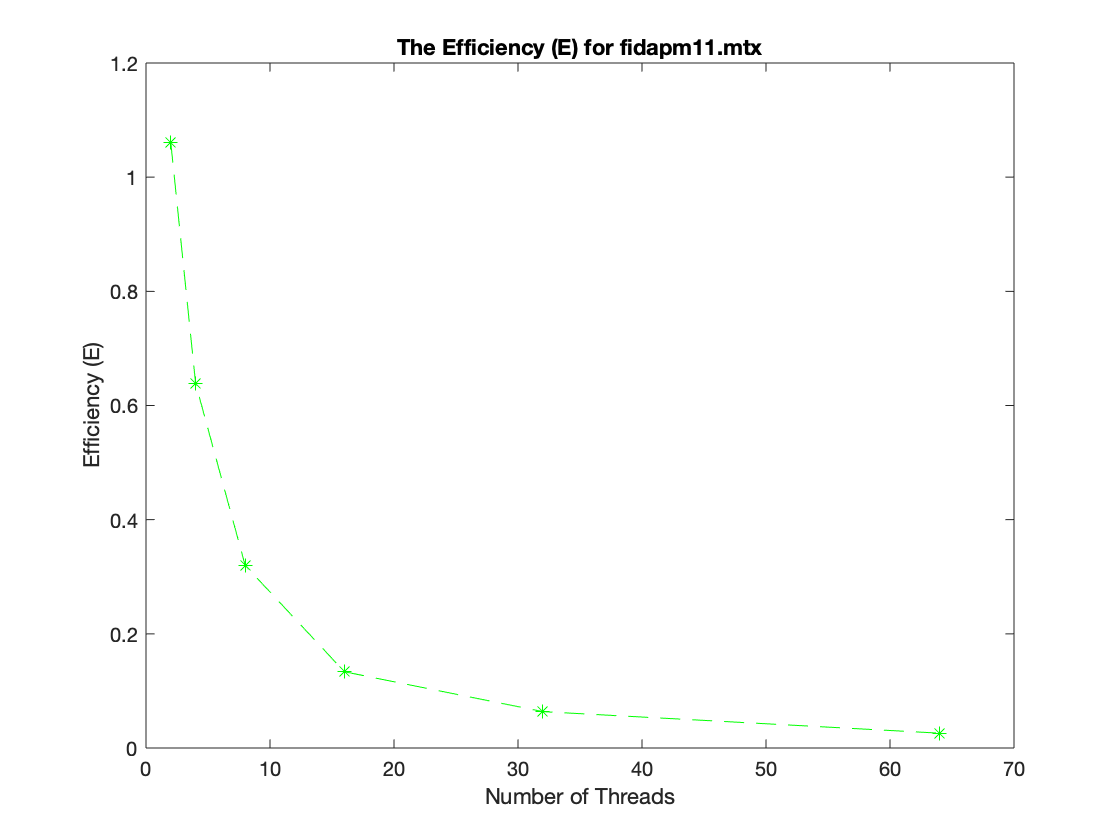
\includegraphics[width=0.75\textwidth]{e2}
    \caption{The efficiency E on test-matrix "fidapm11.mtx" where number of threads for parallel execution is between 2 and 64.}
\end{figure}

\FloatBarrier
\subsection{The parallel running time, speedup, and efficiency of my OpenMP implementation for test-matrix "cavity02.mtx"}

\begin{figure}[!htb]
    \centering
    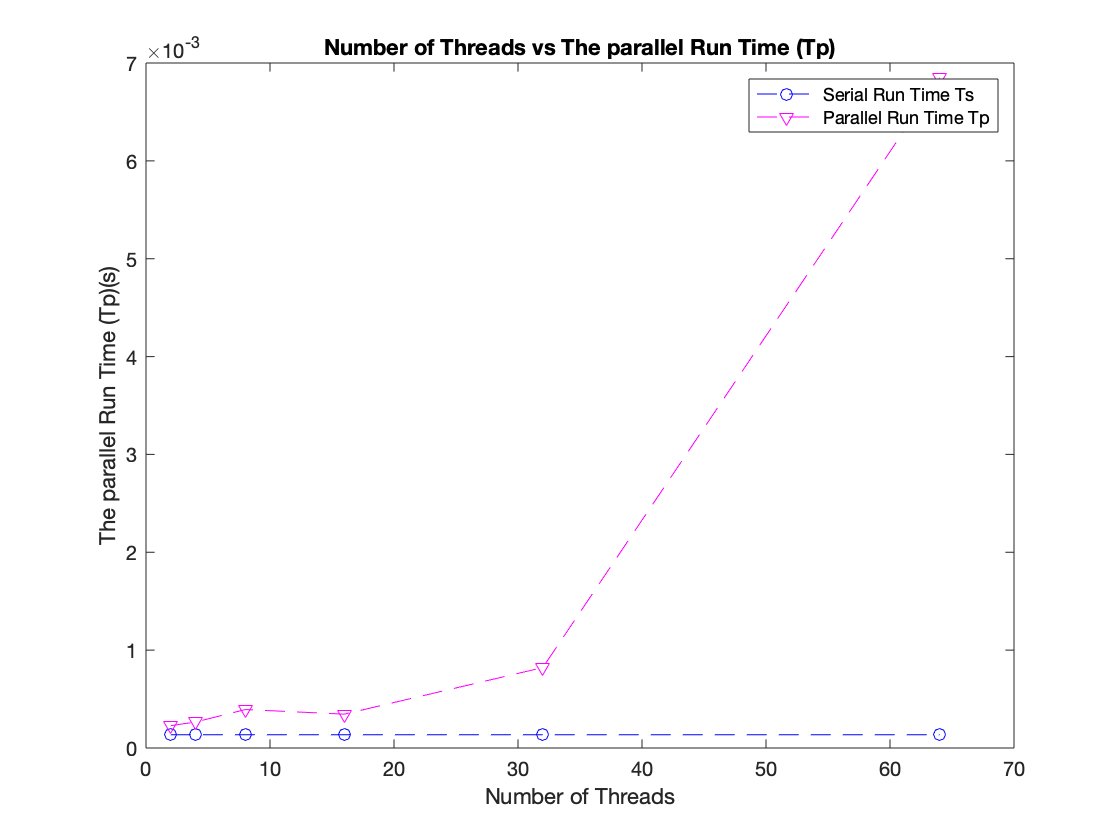
\includegraphics[width=0.75\textwidth]{f3}
    \caption{Serial vs Parallel Run-time comparison of sparse matrix vector multiplication on test-matrix "cavity02.mtx" where number of threads for parallel execution is between 2 and 64.}
\end{figure}

\begin{figure}[!htb]
    \centering
    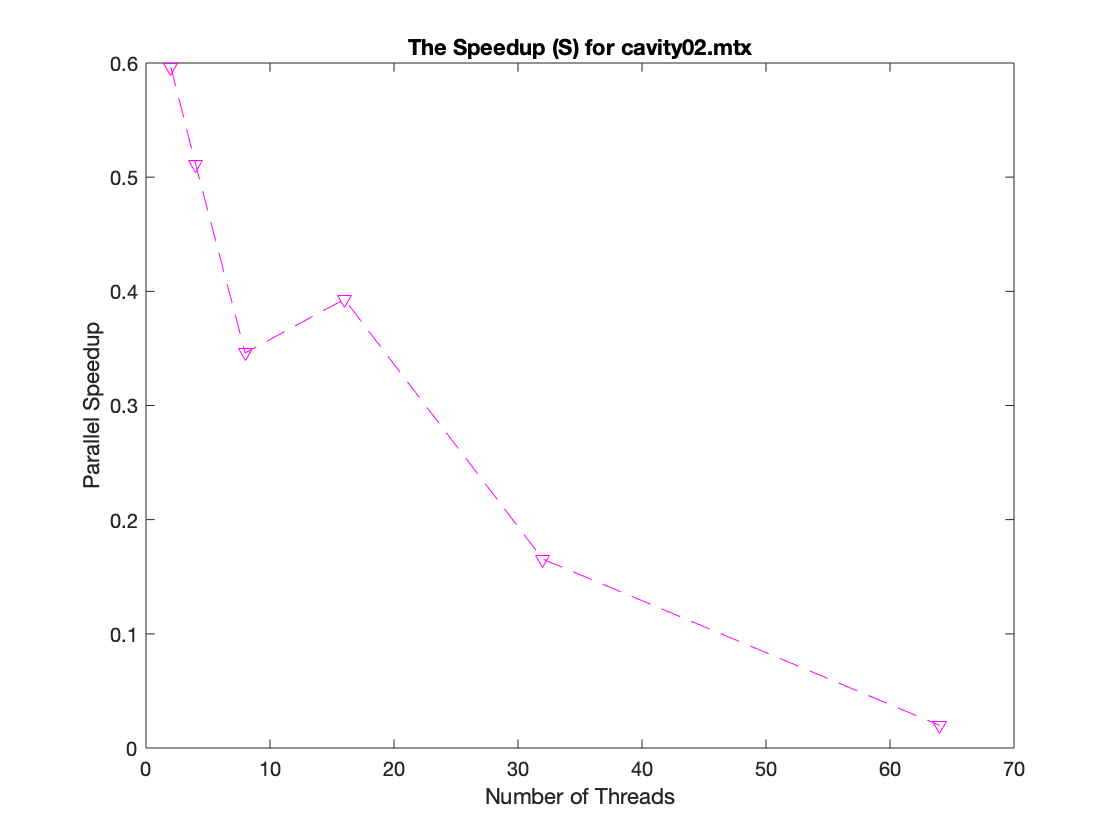
\includegraphics[width=0.75\textwidth]{s3}
    \caption{The speedup S on test-matrix "cavity02.mtx" where number of threads for parallel execution is between 2 and 64.}
\end{figure}

\begin{figure}[!htb]
    \centering
    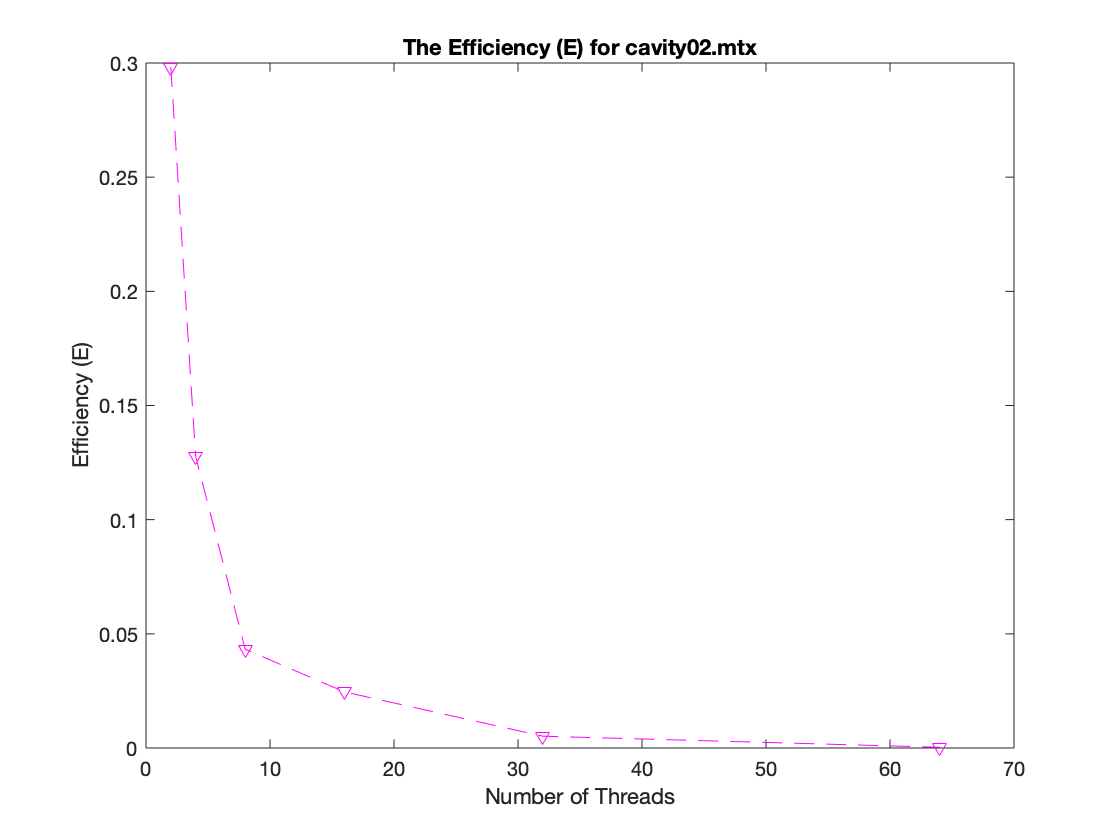
\includegraphics[width=0.75\textwidth]{e3}
    \caption{The efficiency E on test-matrix "cavity02.mtx" where number of threads for parallel execution is between 2 and 64.}
\end{figure}

\FloatBarrier
\section{Results \& Discussion}

With respect to the parallel time, speedup and efficiency results shown in the figures above for three distinct test matrices I will discuss the performance and scalability of the algorithm. Note that the algorithm may have different performance on different parallel architecture.

First of the the data shown in the figures was obtained by running the program with the following arguments;

\centerline{\textbf{./exe 'no\_of\_threads' '1' '0' 'filename'}}

where no\_of\_threads was valued between 2-64 and the number of iterations were fixed as one.
\newline
\newline
The parallel run time is defined as the time that elapses from the moment that a parallel computation starts to the moment that the last processor finishes execution which was measured from the start of the multiplication to the end discarding the file reading. As it can be seen from figures 1,4,7 almost in every execution the parallel run time was faster than the serial execution for each test matrix. Only during the execution with 64 threads the execution in the first and third matrix exceeded the serial execution which can be explained by the fact of communication overheads. Since the number of iteration was fixed as one separating the process into 64 threads increased this overhead. Also from another perspective the size of the first and the third matrix compared to the second one which is almost 70x bigger than the third matrix is also another factor. As size increases the values differ as it can be seen from the figures.
\newline
\newline
The speedup is defined as the ratio of the serial runtime of the best sequential algorithm for solving a problem to the time taken by the parallel algorithm to solve the same problem on p processors.

\begin{equation}
   S = \frac{T_s}{T_p}
\end{equation}

According to figures 2,5,8 the speedup initially increases in the first two figures and then starts decreasing. In a typical algorithm as the number of processors increase the speedup could be negative, sub-linear, linear, super-linear. As it can be seen for the initial executions the speedup follows a super-linear path which was caused by the optimization of the CRS format to store the sparse matrix which indicates that the parallel version does less work than corresponding serial algorithm. Afterwards for a typical success scenario it was expected that the curve to stabilize and take a constant value however, in this case it starts to decrease. This again could be related to the fact that number of iterations is one.
\newline
\newline
The efficiency is defined as the ratio of speedup to the number of processors. Efficiency measures the fraction of time for which a processor is usefully utilized.

\begin{equation}
   E = \frac{S}{p}
\end{equation}

For the first and the second matrices the efficiency starts as approximately to one and decreases in a linear fashion with respect to the speedup values. In all three test matrices this is common however, in the third matrix efficiency starts from 0.3. Since the number of iterations is set as one this effects the efficiency of the program as well.
\newline
\newline
In terms of the scalability of the solution the fact that
\begin{itemize}
    \item \textbf{Increase number of processors ‐‐> decrease efficiency}
    \item \textbf{Increase problem size ‐‐> increase efficiency}
\end{itemize}

This can be clearly seen from the figures since the matrix with the smallest size performed the worst whereas the matrix with the largest size performed the most optimal. Also increasing the number of the threads decreased efficiency which could also seen from the figures. Overall however, a scalable parallel system can always be made cost‐optimal by adjusting the number of processors and the problem size.
\end{document}

